

\begin{center}
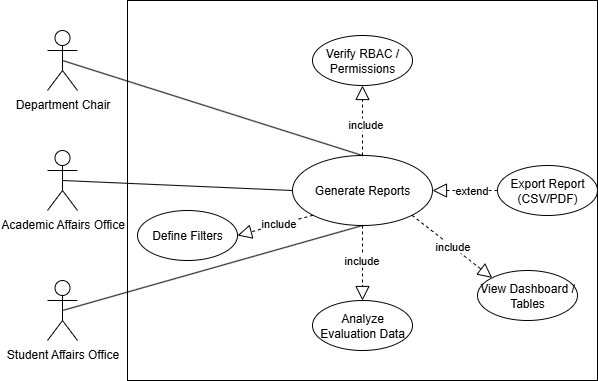
\includegraphics[width=0.9\linewidth]{images/UC-05.png}
\end{center}

\begin{center}
\textbf{Figure 6:}  Reporting \& Analytics
\end{center}

\begin{table}[h!]
\centering
\begin{tabular}{|p{3cm}|p{11cm}|}
\hline
\textbf{Use-case ID} & UC-05 \\
\hline
\textbf{Use-case name} & Reporting \& Analytics \\
\hline
\textbf{Use-case overview} & To allow academic units to view, analyze, and export reports (attendance, performance, tutor workload, student demand, participation) for monitoring and decision-making. \\
\hline
\textbf{Actors} & Department Chair (primary), Academic Affairs Office (primary), Student Affairs Office (primary) \\
\hline
\textbf{Preconditions} & 
1. The user is authenticated via SSO and authorized to view reports. \newline
2. Session, feedback, and progress data exist. \newline
3. The system is operational. \\
\hline
\textbf{Trigger} & Users open the ``Reporting'' module. \\
\hline
\textbf{Steps} & 
1. Retrieve the Reporting page. \newline
2. Select a report type (Departmental / Workload \& Demand / Participation). \newline
3. Set filters (term/date range, department/program, tutor, cohort). \newline
4. Retrieve relevant data and analyze metrics (attendance, performance ratings, tutor workload, student demand, participation). \newline
5. Display dashboards/tables with results and data-source notes. \newline
6. Optional: export the report as CSV or PDF; add metadata (generation time, filters, version) and record the action in the audit log. \\
\hline
\textbf{Postconditions} & 
1. The report is displayed with analyzed metrics. \newline
2. If exported, a CSV/PDF file is produced with metadata. \newline
3. Access/export actions are logged. \\
\hline
\textbf{Exception Flow} & 
1. Access denied: insufficient permissions → show denial message and log the attempt. \newline
2. Invalid/empty filters → show ``No data'' and allow the actor to adjust filters. \newline
3. Export error: I/O or file-size issue → show an error and suggest retrying or narrowing scope. \\
\hline
\end{tabular}
\caption{Use Case UC-05: Reporting \& Analytics}
\end{table}
